\documentclass[aspectratio=169]{beamer}

\title{On Elementary Properties of a Multidimensional Generalization of the Euclidean Algorithm}
\author{Daniel Knaack}
\date{}

\usepackage{tikz}
\usepackage{fontspec}
\usepackage{unicode-math}
\usepackage{standalone}
\usepackage{adjustbox}

\setmathfont{TeX Gyre Pagella Math}
\usetikzlibrary{decorations.pathreplacing, calligraphy, intersections, backgrounds, graphdrawing, graphs, calc, 3d}
\tikzset{>=stealth}

\newtheorem{conjecture}{Conjecture}

\usetheme{metropolis}
\usefonttheme[onlymath]{serif}
\setbeamertemplate{caption}{\raggedright\insertcaption\par}

\begin{document}

\begin{frame}
  \maketitle
\end{frame}

\begin{frame}
  \begin{itemize}
    \item A number is rational if and only if its decimal expansion is eventually periodic
    \item A number is a quadratic irrational if and only if its continued fraction expansion is eventually periodic
    \item A number is a cubic irrational if and only if ?
  \end{itemize}
\end{frame}

\begin{frame}
  \begin{problem}[Hermite, 1839]
    Does there exist a representation of the real numbers as a sequence of
    integers such that the representation is eventually periodic if and only if
    the number is \alt<2>{an algebraic number of degree $d$}{a cubic irrational}?
  \end{problem}
\end{frame}

\begin{frame}
  \frametitle{Outline}
  \small
  \begin{columns}
    \column{0.49\textwidth}
    \textbf{Quadratic Irrationals}:
    \begin{enumerate}
      \item The Euclidean Algorithm
      \item Fibonacci Numbers
      \item Continued Fractions
      \item Periodicity and Quadratic Irrationals
    \end{enumerate}

    \column{0.49\textwidth}
    \textbf{Algebraic Numbers}:
    \begin{enumerate}
      \item The Generalized Euclidean Algorithm
      \item Higher-Order Fibonacci Numbers
      \item Multidimensional Continued Fractions
      \item Periodicity and Algebraic Numbers?
    \end{enumerate}
  \end{columns}
\end{frame}

\begin{frame}
  \frametitle{The Euclidean Algorithm}
  \small
  \begin{columns}[T]
    \column{0.45\textwidth}
    \begin{problem}[Greatest Common Divisor]
      \begin{itemize}
        \item \textbf{Input}: $a, b ∈ ℤ$.
        \item \textbf{Output}: $c = \gcd(a, b)$.
      \end{itemize}
    \end{problem}
    % TODO: Zahlenstrahl
    \column{0.45\textwidth}
    \begin{problem}[Lattice Basis Computation]
      \begin{itemize}
        \item \textbf{Input}: $A ∈ ℤ^{d×n}$ with $n > d$.
        \item \textbf{Output}: $B ∈ ℤ^{d×d}$ such that \[\mathcal L(B) = \mathcal L(A).\]
      \end{itemize}
    \end{problem}
  \end{columns}
  \begin{columns}
    \column{0.49\textwidth}
    \begin{center}
      \begin{tikzpicture}
        \draw[->] (-2, 0) -- (2, 0) node[right] {$ℤ$};

        \draw (-1.5, 0.1) -- (-1.5, -0.1) node[below] {$0$};
        \draw (0.5, 0.1) -- (0.5, -0.1) node[below] {$a$};
        \draw (1, 0.1) -- (1, -0.1) node[below] {$b$};
      \end{tikzpicture}
    \end{center}

    \column{0.49\textwidth}
    \begin{center}
      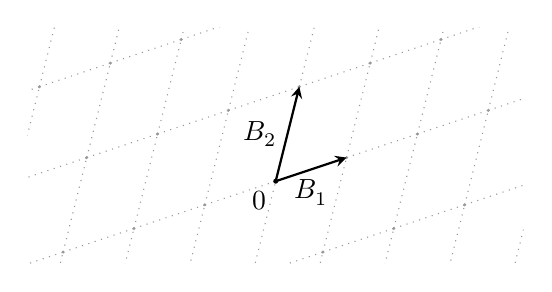
\begin{tikzpicture}[scale=0.3]
        \clip (-10.5, -3.5) rectangle (10.5, 6.5);

        \foreach \x in {-10,...,10}
        \foreach \y in {-10,...,10}
        {
          \draw[black!40, dotted] (3*\x + \y, \x + 4*\y) -- (3*\x + \y + 1, \x + 4*\y + 4);
          \draw[black!40, dotted] (3*\x + \y, \x + 4*\y) -- (3*\x + 3 + \y, \x + 1 + 4*\y);
          \fill[black!40] (3*\x + \y, \x + 4*\y) circle (2pt);
        }

        \draw[->, thick] (0, 0) -- node[below] {$B₁$} (3, 1);
        \draw[->, thick] (0, 0) -- node[left] {$B₂$} (1, 4);
        \fill (0, 0) circle (3pt) node[below left] {$0$};
      \end{tikzpicture}
    \end{center}
  \end{columns}
\end{frame}

\begin{frame}[fragile]
  \frametitle{Modulo}
  \begin{columns}
    \column{0.49\textwidth}
    \includestandalone{figures/golden-rectangle}

    \column{0.49\textwidth}
    \adjustbox{scale=0.7}{\includestandalone{figures/lattice-modulo}}
  \end{columns}
\end{frame}

\begin{frame}
  \frametitle{Fibonacci Numbers}
\end{frame}

\begin{frame}
  \frametitle{Continued Fractions}
  \small
  \begin{columns}[T]
    \column{0.49\textwidth}
    A continued fraction over a sequence over integers $(aₙ)_{n≥0}$ is defined as
    \[
      [a₀; a₁, …] = a₀ + \frac{1}{[a₁; a₂, …]}.
    \]

    \column{0.49\textwidth}
    A \emph{multidimensional continued fraction} over a sequence over integer
    vectors $(a^{(n)})_{n≥0}$ is defined as
    \[
      [a^{(0)}; a^{(1)}, …] = \mathrm{pivot}^{-1}(a^{(0)}, [a^{(1)}; a^{(2)}, …]).
    \]
  \end{columns}
\end{frame}

\begin{frame}
  \frametitle{Geometry}

  \begin{columns}
    \column{.49\textwidth}
    \[
      p/q ↦ \begin{pmatrix}
        p \\
        q \\
      \end{pmatrix}
    \]
    %\adjustbox{scale=.9}{\includestandalone{figures/klein-polygon}}

    \column{.49\textwidth}
    \[
      (p₁/q, …, p_d/q) ↦ \begin{pmatrix}
        q   \\
        p_1 \\
        ⋮   \\
        p_d \\
      \end{pmatrix}
    \]
    %\adjustbox{scale=.9}{\includestandalone{figures/projective-space}}
  \end{columns}
\end{frame}

\begin{frame}
  % TODO: Figure for pivot rule
  \[
    x_i' =
    \begin{cases}
      \frac{1}{x_ℓ - a_ℓ}, & \text{ if } i = ℓ, \\
      \frac{x_i - a_i}{x_ℓ - a_ℓ}, & \text{ otherwise},
    \end{cases}
    \iff
    x_i =
    \begin{cases}
      a_ℓ + \frac{1}{x_ℓ'}, & \text{ if } i = ℓ, \\
      a_i + \frac{x_i'}{x_ℓ'}, & \text{ otherwise}.
    \end{cases}
  \]
\end{frame}

\begin{frame}
  \frametitle{Convergence}
  \small
  \begin{columns}[T]
    \column{0.49\textwidth}
    \begin{theorem}
      Let $pₙ/qₙ$ be the convergent of a continued fraction for $x ∈ ℝ$.
      Then,
      \[
        \left|x - \frac{pₙ}{qₙ}\right| < \frac{1}{qₙ^2}.
      \]
    \end{theorem}

    \column{0.49\textwidth}
    \begin{theorem}
      The convergents $r^{(n)}$ of a multidimensional continued fraction approach $x ∈ ℝ^d$, if
      \begin{enumerate}
        \item Every index is used infinitely often
        \item The distance between two equal indices is constant.
      \end{enumerate}
    \end{theorem}
  \end{columns}
\end{frame}

\begin{frame}
  \begin{center}
    \includestandalone{figures/projective-space}
  \end{center}
\end{frame}

\begin{frame}
  \frametitle{Periodicity $\Rightarrow$ Algebraicity}
  \small
  \begin{columns}[T]
    \column{0.49\textwidth}
    \begin{theorem}
      If a continued fraction of a number $x ∈ R$ is periodic, then $x$ is a
      quadratic irrational.
    \end{theorem}

    \begin{proof}[Proof Sketch]
      If the continued fraction is periodic,
      then $(x, 1)$ is the eigenvector of an integer matrix $B ∈ ℤ^{2×2}$.
    \end{proof}

    \column{0.49\textwidth}
    \begin{theorem}
      If a multidimensional continued fraction of a vector $x ∈ ℝ^d$ is
      periodic, then $[ℚ(x₁, …, x_d) : ℚ] ≤ d+1$.
    \end{theorem}

    \begin{proof}[Proof Sketch]
      If the continued fraction is periodic,
      then $(x, 1)$ is the eigenvector of an integer matrix $B ∈ ℤ^{(d+1)×(d+1)}$.
    \end{proof}
  \end{columns}
\end{frame}

\begin{frame}
  \frametitle{Periodicity $\Leftarrow$ Algebraicity}
  \small
  \begin{columns}[T]
    \column{0.49\textwidth}
    \begin{theorem}
      If $x$ is a quadratic irrational,
      then its continued fraction is periodic.
    \end{theorem}

    \begin{proof}[Proof Sketch]
      For every quadratic irrational,
      there exists a matrix $U ∈ ℤ^{2×2}$, which preserves the Klein polygon and thus, the convergents.
    \end{proof}

    \column{0.49\textwidth}
    \begin{conjecture}
      If $x$ is an algebraic number of degree $d+1$,
      then the multidimensional continued fraction of $(x^1, …, x^d)$ is
      periodic.
    \end{conjecture}
  \end{columns}
\end{frame}

\begin{frame}
  \small
  \begin{columns}
    \column{0.49\textwidth}
    \begin{enumerate}
      \item The Euclidean Algorithm
      \item Fibonacci Numbers
      \item Continued Fractions
      \item Periodicity and Quadratic Irrationals
    \end{enumerate}

    \column{0.49\textwidth}
    \begin{enumerate}
      \item The Generalized Euclidean Algorithm
      \item Higher-Order Fibonacci Numbers
      \item Multidimensional Continued Fractions
      \item Periodicity and Algebraic Numbers?
    \end{enumerate}
  \end{columns}
\end{frame}

\end{document}
